\documentclass{beamer}

\usepackage[utf8]{inputenc}
\usepackage[english]{babel}
\usepackage[T1]{fontenc}
\usepackage{lmodern}
\usepackage{adjustbox}
\usepackage{graphicx}
\usepackage{caption}
\usepackage{subcaption}
\usepackage{color, colortbl}
\usepackage{commath}
\usepackage{amsmath,amssymb,amsthm}
\usepackage{tikz}
\usepackage{pgffor}
\usepackage{enumitem}
\DeclareMathOperator*{\argmax}{arg\,max}
\DeclareMathOperator*{\argmin}{arg\,min}
\usepackage[lined]{algorithm2e}
\usetheme{Singapore}
\newlength{\mylen}
\resetcounteronoverlays{compt}
\addtobeamertemplate{navigation symbols}{}{%
    \usebeamerfont{footline}%
    \usebeamercolor[fg]{footline}%
    \hspace{1em}%
    \insertframenumber/\inserttotalframenumber
}
\usepackage{upgreek}
\usepackage[doi=false,
            isbn=false,
            url=false,
            bibstyle=authoryear,
            style=authoryear]{biblatex}
\bibliography{biblio}%
\renewcommand{\footfullcite}[1]{\footnote[frame]{\fullcite{#1}}}
\def\bibfont{\tiny}%
\begin{document}

\title{Viterbi Algorithm for Intrusion Type Identification in Anomaly
  Detection System}
\author{ } 
\institute{ }
\date{january 14th 2019}

\maketitle

\section{Introduction}

\begin{frame}
\frametitle{Context}
\end{frame}

\begin{frame}
  \frametitle{Intrusion Type}
  \begin{itemize}[label=.]
  \item Buffer overflow
    \begin{itemize}[label=.]
    \item xlock vulnerability
    \item lpset vulnerability
    \item kcms\_sparc vulnerability
    \end{itemize}
  \item S/W security vulnerability
  \item Setup vulnerability
  \item Denial of service
  \end{itemize}
\end{frame}

\section{Backgroung}
\begin{frame}
  \frametitle{Markov Chain}
  \begin{columns}[T]
    \begin{column}{.7\textwidth}
      A markov Chain is defined by :
      \begin{itemize}[label=.]
      \item S, A finite set of N states
      \item $\pi$, A vector of initial probabilities over S :
        $$\pi_i = P(S_1 = i), 1 \leq i \leq N$$
      \item A, A matrix of probabilities of transitions over $SxS$ :
        $$a_{ij} = P(S_t = j | S_{t-1} = i), 1 \leq i \leq N$$
      \item Markov assumption :
        $P(S_t|S_{t-1},S_{t-2},\ldots,S_{1})=P(S_t|S_{t-1})$ 
      \end{itemize}
    \end{column}
    \begin{column}{.28\textwidth}
      \begin{figure}
        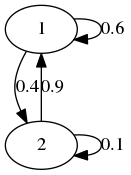
\includegraphics[scale=0.4]{img/markov_chain_example.png}
        $$
        A = \begin{pmatrix}
          0.6 & 0.4 \\
          0.9 & 0.1
        \end{pmatrix}
        $$
        \caption{Simple example of Markov Chain}
      \end{figure}
    \end{column}
  \end{columns}
\end{frame}

\begin{frame}
  \frametitle{HMM - Hidden Markov Model}
  \begin{itemize}[label=--]
  \item Hidden Markov Model is a statistical model in which the
    modeled system is supposed to be a Markovian process of unknown
    parameters.\pause
  \item Hidden Markov Model can be viewed as a Bayesian Network\pause
  \item We define a HMM including :
    \begin{itemize}
    \item V, A finite set of M observations
    \item B, A a matrix of probabilities of observations
      over state :
      $$b_i(k) = P(0_t=V_k | S_t = i)$$
    \end{itemize}
  \end{itemize}
\end{frame}

\begin{frame}
  \frametitle{HMM - Forward Algorithm}
  \scalebox{0.7}{
    \begin{algorithm}[H]
      \SetKwInOut{Input}{input }
      \SetKwInOut{Output}{output }
      \Input{$\lambda$ The model, $O$ Observed sequence}
      \Output{ $P(0|\lambda)$}
      Step 1, Initialization :
        $
        \forall i, \alpha_1(i) = \pi_i b_i(0_1)
        $\\
        Step 2, Induction :\\
        \For{$t\gets2:T$}{
          $
          \forall in \alpha_t(i) = \left[ \sum\limits_{j=1}^N\alpha_{t-1}(i)a_{ij}\right]
          b_j(O_t)
          $
        }
        Step 3, Termination :
        $
        P(0|\lambda) = \sum\limits_{i=1}^N \alpha_t(i)
        $
    \end{algorithm}
  }
  \footfullcite{forward_algo}
\end{frame}

\begin{frame}
  \frametitle{HMM - Viterbi Algorithm}
  \scalebox{0.6}{
    \begin{algorithm}[H]
      \SetKwInOut{Input}{input }
      \SetKwInOut{Output}{output }
      \Input{$O$ Observed sequence}
      \Output{ $\argmax\limits_{\lambda \in \Lambda} P(0|\lambda)$}
      Step 1, Initialization :\\
      \For{$i\gets1:N$}{
        $\delta_1(i) = \pi_i b_i(0_1)$\\
        $\psi_1(i) = 0$
      }
      Step 2, Recursion :\\
      \For{$t\gets2:T$}{
        \For{$j\gets1:N$}{
          $\delta_t(j) = \max\limits_i [\delta_{t-1}(i)a_{ij}]b_j(0_t)$\\
          $\psi_t(j) = \argmax\limits_i [\delta_{t-1}(i)a_{ij}]b_j(0_t)$
        }
      }
      Step 3, Termination :\\
      $P^{*} = \max\limits_{s \in S}[\delta_T(s)]$\\
      $S_T^{*} = \argmax\limits_{s \in S}[\delta_T(s)]$\\
      Step 4, Backtracking :\\ 
      \For{$t\gets{T-1}:1$}{
        $S_t^{*} = \psi_{t+1}(s_{t+1 }^{*})$
      }
      \Return{$S^{*}$}
    \end{algorithm}
        }
        \footfullcite{viterbi}
\end{frame}
\section{Proposed Method}
\subsection{Intrusion Detection}
\begin{frame}
  \frametitle{Normal Behaviour Modeling}
  \begin{itemize}
  \item Normal Behaviour is modelised by a left-to-right HMM $\lambda$.
  \item The forward allgorithm is used to decide whether normal or not
    with a threshold.
  \end{itemize}
\end{frame}
\begin{frame}
  \frametitle{Intrusion Detection}
  \framesubtitle{Initialization}
  Show Example
\end{frame}
\begin{frame}
  \frametitle{Intrusion Detection}
  \framesubtitle{Induction}
  Show Example
\end{frame}
\begin{frame}
  \frametitle{Intrusion Detection}
  \framesubtitle{Termination}
  Show Example
\end{frame}
\begin{frame}
  \frametitle{Intrusion Detection}
  \framesubtitle{Decision}
  \scalebox{1}{
    \begin{algorithm}[H]
      \uIf{$log(P(0|\lambda)) >~thresold$}{
        \Return{Normal Behaviour} 
      }
      \Else{
        \Return{Intrusion}
      }
    \end{algorithm}
    }
  \\Show Example
\end{frame}
\begin{frame}
  \frametitle{Intrusion Detection}
  \framesubtitle{Results}
  \begin{table}[h]
    \centering
    \caption{\label{tab:IDS}The performance of HMM-based IDS. Best
      results are in bold}
    \begin{tabular}{|c |c | c | c |}
      \hline
      Length & Thresold & Detection Rate & F-P Error \\ \hline
      10 & -9.43 & 100\% & 2.626 \\ \hline
      15 & -9.43 & 100\% & 3.614 \\ \hline
      10 & -14.42 & 100\% & 1.366 \\ \hline
      15 & -14.42 & 100\% & 2.718 \\ \hline
      10 & -16.94 & 100\% & 0.789 \\ \hline
      15 & -16.94 & 100\% & 2.618 \\ \hline
      10 & -18.35 & 100\% & 0.553 \\ \hline
      15 & -18.35 & 100\% & 2.535 \\ \hline
      10 & -19.63 & 100\% & 0.476 \\ \hline
      15 & -19.63 & 100\% & 2.508 \\ \hline
      \textbf{10} & \textbf{-20.83} & \textbf{100\%} & \textbf{0.372}
      \\ \hline
      15 & -20.83 & 100\% & 2.473 \\ \hline
    \end{tabular}
  \end{table}    
\end{frame}
\subsection{Intrusion Type Identification}
\begin{frame}
  \frametitle{Intrusion Type Identification}
  Process in two steps :
  \begin{itemize}
  \item Viterbi algorithm used to find the optimal state sequence
  \item Euclidiant distance to identify the intrusion type with the
    optimal state sequence
  \end{itemize}
\end{frame}
\begin{frame}
  \frametitle{Intrusion Type Identification}
  \framesubtitle{Initialization}
  Show Example
\end{frame}
\begin{frame}
  \frametitle{Intrusion Type Identification}
  \framesubtitle{Recursion}
  Show Example
\end{frame}
\begin{frame}
  \frametitle{Intrusion Type Identification}
  \framesubtitle{Termination}
  Show Example
\end{frame}
\begin{frame}
  \frametitle{Intrusion Type Identification}
  \framesubtitle{Backtracking}
  Show Example
\end{frame}
\begin{frame}
  \frametitle{Intrusion Type Identification}
  \framesubtitle{Decision}
  Show Example
\end{frame}
\begin{frame}
  \frametitle{Intrusion Type Identification}
  \framesubtitle{Results}
  \begin{table}[h]
    \centering
    \caption{\label{tab:IDS}The performance of Viterbi-based Intrusion
      Type Identification}
    \begin{tabular}{|c| c|c | c | c |}
      \hline
      Attack & Trial & Correct & Incorrect & Rate \\ \hline
      Buffer Overflow & 20 & 18 & 2 & 90\% \\ \hline
      Denial of Service & 25 & 9 & 16 & 36\% \\ \hline
      Buffer Overflow & 45 & 27 & 18 & 60\% \\ \hline
    \end{tabular}
  \end{table}    
\end{frame}

\section{Limitations \& Remarks}
\begin{frame}
  \frametitle{Limitations \& Remarks}
  \begin{itemize}
  \item Try other distance metrics for Intrusion Type Identification :
    \fullcite{10.1007/11590316_30}\pause
  \item Bad results for Denial of Service :
    \fullcite{7366308}
  \end{itemize}
\end{frame}

\section{Other Method}
\begin{frame}
  \frametitle{Methods using HMM}
\end{frame}

\begin{frame}
  \frametitle{Other Methods}
  %\footfullcite{Buczak2016ASO}
\end{frame}

\end{document}
